% arara: clean: {
% arara: --> extensions:
% arara: --> ['aux', 'bbl', 'bcf', 'blg', 'log', 'nav',
% arara: --> 'out', 'pdf', 'run.xml', 'snm', 'toc', 'vrb']
% arara: --> }
% arara: lualatex: {
% arara: --> shell: yes,
% arara: --> draft: yes,
% arara: --> interaction: batchmode
% arara: --> }
% arara: biber
% arara: lualatex: {
% arara: --> shell: yes,
% arara: --> draft: no,
% arara: --> interaction: batchmode
% arara: --> }
% arara: lualatex: {
% arara: --> shell: yes,
% arara: --> draft: no,
% arara: --> interaction: batchmode
% arara: --> }
% arara: clean: {
% arara: --> extensions:
% arara: --> ['aux', 'bbl', 'bcf', 'blg', 'log', 'nav',
% arara: --> 'out', 'run.xml', 'snm', 'toc', 'vrb']
% arara: --> }
\documentclass[
    8pt,
    aspectratio=1610,
    c,
    % handout,
    intlimits,
    leqno,
    professionalfonts,
    spanish,
    xcolor=svgnames
]{beamer}

\usepackage[spanish]{babel}
\usepackage{mathtools}
\usepackage{diffcoeff}
\usepackage{minted}
\usepackage[
    linesnumbered,
    ruled,
    % boxed,
    vlined,
    spanish
]{algorithm2e}
\usepackage{algorithmicx}
\usepackage[
    backend=biber,
    defernumbers=true,
    firstinits=true,
    citestyle=numeric,
    bibstyle=numeric,
    sorting=nty
]{biblatex}

\usefonttheme[onlymath]{serif}
\setbeamercolor{structure}{fg=DarkBlue}
\setbeamercovered{transparent}
\setbeamerfont{block title}{size={\centering\normalsize}}
\setbeamerfont{normal text}{size=\small}
\setbeamerfont{section in toc}{size=\normalsize,series=\bfseries,family=\sffamily}
\setbeamersize{text margin left=8pt,text margin right=8pt}
\setbeamertemplate{footline}[frame number]{}
\setbeamertemplate{frametitle}[default][center]
\setbeamertemplate{headline}{}
\setbeamertemplate{itemize items}[circle]
\setbeamertemplate{navigation symbols}{}
\setbeamertemplate{theorems}[ams style]
\addtobeamertemplate{theorem begin}{\normalfont}{}
\addbibresource{references.bib}

\title{\bfseries\sffamily Künstliche neuronale Netze}
\subtitle{\color{DarkRed}Einführung in die Numerische Mathematik}
\institute{Traducción al español por Carlos Aznarán}
\author{Thomas Richter\qquad\and\qquad Henry von Wahl\qquad\and\qquad\color{DarkBlue}Thomas Wick}
\date{\today}
\titlegraphic{
    \begin{picture}(0,0)
        \put(-130,80){\makebox(0,0)[rt]{\href{https://link.springer.com/book/10.1007/978-3-662-69582-1}{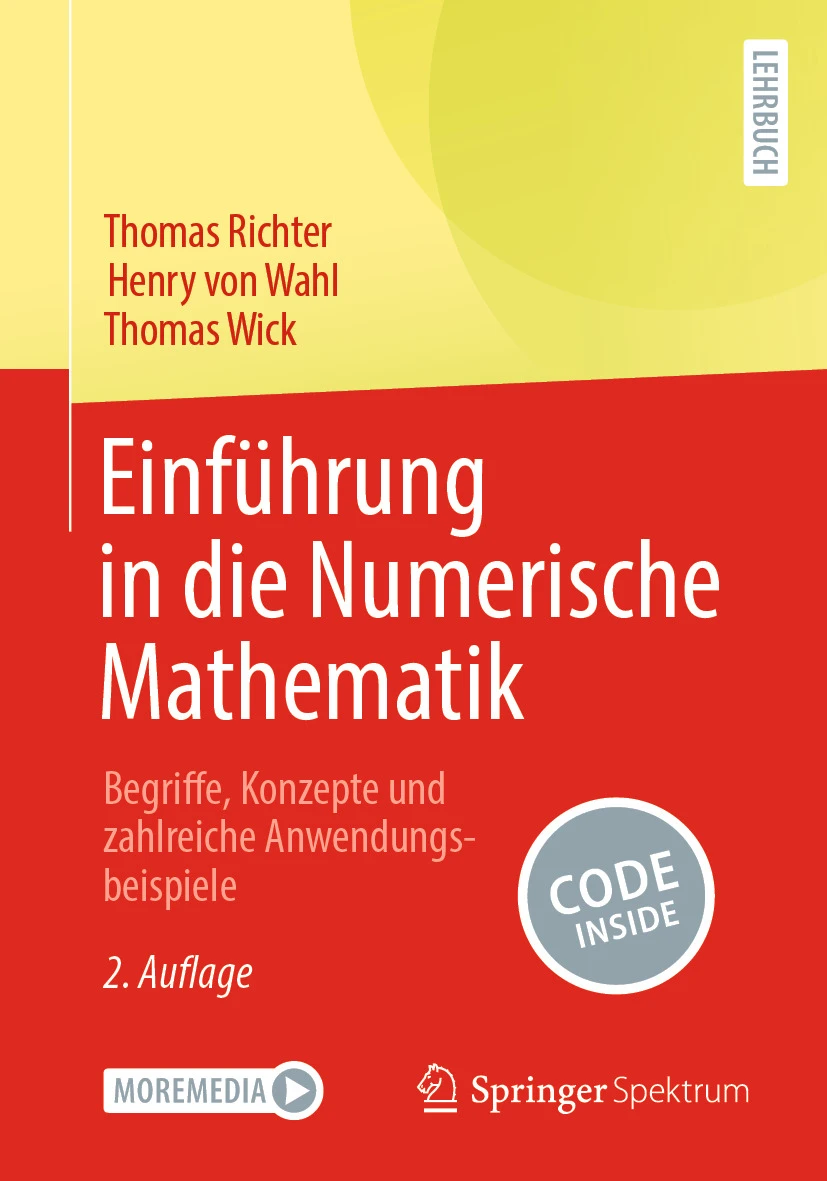
\includegraphics[width=2.5cm]{einführung}}}}
        \put(200,80){\makebox(0,0)[rt]{\href{http://thomaswick.org}{
\includegraphics[width=2.5cm]{wick}}}}
    \end{picture}
}

\begin{document}

\frame{
  \maketitle
}

\begin{frame}
  \frametitle{\bfseries\sffamily Redes Neuronales Artificiales}

  Matemáticamente hablando, las \alert{redes neuronales artificiales}
  (RNA) son funciones compuestas por bloques de construcción muy
  simples con una gran cantidad de parámetros libres.
  Estos parámetros pueden especificarse para que la red neuronal
  artificial realice una tarea matemática específica, lo que
  significa simplemente que se aproxima a una función que determina
  el resultado de la tarea.
  Por lo tanto, el \alert{aprendizaje automático}, y en particular el
  trabajo con redes neuronales artificiales, puede considerarse un
  tipo de aproximación.
  Sin embargo, a diferencia de la interpolación polinómica o
  trigonométrica, el \alert{aprendizaje automático} con
  \alert{redes neuronales artificiales} utiliza un tipo de función
  completamente diferente.
  En este caso, no se elige un espacio vectorial estructurado, como el
  espacio de polinomios o polinomios trigonométricos, para aproximar
  una función, sino que se ensamblan funciones a partir de componentes
  elementales: las neuronas artificiales.

  \pause

  \

  Inicialmente, la investigación matemática sobre redes neuronales
  artificiales se inspiró en sus contrapartes naturales, es decir, en
  el funcionamiento de las neuronas cerebrales.
  Hoy en día, constituyen una herramienta enormemente poderosa que
  puede utilizarse de forma muy eficiente en los ordenadores modernos.
  Muchos problemas antiguos se han resuelto finalmente con éxito
  gracias a las redes neuronales artificiales.
  Cabe destacar los avances en el procesamiento del lenguaje, como la
  traducción automática, el reconocimiento de voz y los modelos de
  lenguaje generativo como ChatGPT, así como los importantes logros
  en el procesamiento de imágenes y vídeos.

  \pause

  \

  Matemáticamente, podemos considerar las redes neuronales
  artificiales como un método para aproximar funciones.
  Sin embargo, su análisis es más complejo y se carece de muchas
  herramientas: la interpolación de Lagrange se basaba
  principalmente en la expansión de Taylor y la representación del
  polinomio de interpolación con polinomios base.
  Sin embargo, las redes neuronales a menudo no son diferenciables
  ni representan un espacio vectorial con una base.

  \pause

  \

  La mejor aproximación gaussiana es un problema de minimización con
  un funcional cuadrático, que puede resolverse con precisión
  mediante el producto escalar.
  Las redes neuronales también se determinan mediante problemas de
  minimización, pero estas tareas de minimización tienen una
  estructura no lineal compleja, no son cuadráticas y, por lo
  general, no son unívocamente resolubles.
  Por lo tanto, carecen de propiedades estructurales importantes
  para el análisis.
\end{frame}
\section{Construcción de redes neuronales artificiales}

\begin{frame}
    El elemento básico es la neurona artificial y el nombre se basa en
    el funcionamiento de las neuronas en el cerebro:

    \pause

    \begin{definition}[Neurona artificial]
        Sea $w\in\mathbb{R}^{n}$ y $b\in\mathbb{R}$, así como
        $f\colon\mathbb{R}^{n}\to\mathbb{R}$.
        Entonces la función se llama
        \vspace*{-.5\baselineskip}\setlength\belowdisplayshortskip{0pt}
        \begin{equation*}
            f\colon\mathbb{R}^{n}\to\mathbb{R},\quad
            f\left(x\right)=\sigma\left(\sum_{i=1}^{n}w_{i}x_{i}+b\right),
        \end{equation*}
        se denomina \alert{neurona artificial}.
        El vector $w\in\mathbb{R}^{n}$ se denomina peso y
        $b\in\mathbb{R}^{n}$ es el sesgo.
        La función $\sigma\colon\mathbb{R}\to\mathbb{R}$ se denomina
        \alert{función de activación}.
    \end{definition}

    \pause

    No existe una definición clara del término función de activación.
    En cambio, se refiere a una función (no lineal) que determina
    cuándo se activa la salida de una neurona artificial.

    La variante más simple es la función de Heaviside:
    \vspace*{-.5\baselineskip}\setlength\belowdisplayshortskip{0pt}
    \begin{equation*}
        \sigma_{\text{HS}}\left(s\right)=
        H\left(s\right)\coloneqq
        \begin{cases}
            0, & s< 0.   \\
            1, & s\geq0.
        \end{cases}
    \end{equation*}

    Una función de activación continua es la
    \alert{Unidad Lineal Rectificada} (ReLU)
    \begin{equation*}
        \sigma_{\text{ReLU}}\left(s\right)=
        \operatorname{ReLu}\left(s\right)\coloneqq
        \begin{cases}
            0, & s\leq 0. \\
            s, & s>0.
        \end{cases}
    \end{equation*}

    Las \alert{activaciones sigmoideas} son continuamente
    diferenciables (con una frecuencia arbitraria).
    \begin{equation*}
        \sigma\left(s\right)=
        \frac{1}{1+\exp\left(-s\right)},
    \end{equation*}
    o la tangente hiperbólica
    \begin{equation*}
        \sigma_{\tanh}\left(s\right)=
        \tanh\left(s\right).
    \end{equation*}

    Estas dos están estrechamente relacionadas, es
    \vspace*{-.5\baselineskip}\setlength\belowdisplayshortskip{0pt}
    \begin{equation*}
        \sigma\left(s\right)=
        \frac{1}{2}
        \tanh\left(\frac{x}{2}\right)+
        \frac{1}{2}.
    \end{equation*}
\end{frame}

\begin{frame}
    \begin{figure}[ht!]
        \centering
        \includegraphics[width=.7\paperwidth]{1110}
        \caption{Izquierda: Esquema de una neurona artificial con tres
            señales de entrada, la capa lineal y la activación no lineal.
            Derecha: El desarrollo de algunas funciones de activación
            típicas.}
        \label{fig:11.10}
    \end{figure}
    En la Figura~\ref{fig:11.10} mostramos el curso de estas funciones
    de activación así como la estructura esquemática de una neurona
    artificial.

    \pause

    \begin{example}[Clasificación con neuronas artificiales]
        Una neurona artificial con activación de Heaviside
        \vspace*{-.5\baselineskip}\setlength\belowdisplayshortskip{0pt}
        \begin{equation*}
            f\left(x\right)=
            H\left({\left\langle w,x\right\rangle}_{2}+b\right),
        \end{equation*}
        divide el espacio en un hiperplano, porque cada plano con vector
        normal $n$ y punto seleccionado $x_{0}$ está dado por
        \begin{equation*}
            0=n^{T}\left(x-x_{0}\right)=
            n^{T}x-
            n^{T}x_{0}.
        \end{equation*}

        \pause

        Por lo tanto, el peso corresponde al vector normal, y el sesgo es
        el producto escalar con el punto seleccionado.
        Una neurona divide así el espacio en dos mitades más allá del
        plano, y esta es una de las tareas fundamentales para las que se
        pueden utilizar redes neuronales artificiales.
    \end{example}
\end{frame}

\begin{frame}
    Dados $x_{1},\dotsc,x_{N}$, a cada una se le asigna una propiedad
    $y_{i}$, simplemente $y_{i}\in\left\{0,1\right\}$.
    Buscamos los pesos $w$ y el sesgo $b$ de la neurona artificial
    tales que $f\left[w,b\right](x_{i})=y_{i}$.
    Es decir, buscamos un modelo que realice la clasificación de los
    datos en función de las propiedades.
    Los pesos refuerzan o debilitan la influencia de la entrada y, por
    lo tanto, la transición de la no activación de una neurona a la
    activación.
    El sesgo asegura un cambio en la activación.
    Un modelo compuesto por una sola neurona es muy limitado, y debe
    asumirse que la tarea no puede resolverse con exactitud.
    En su lugar, intentamos encontrar el mejor modelo; es decir,
    consideramos el problema de minimización de forma análoga a la
    regresión de la Sección 4.5 y el Excurso 11.4.
    \begin{equation*}
        \min_{\left(w,b\right)}
        \sum_{i=1}^{N}
        {\left\|y_{i}-f\left[w,b\right]\left(x_{i}\right)\right\|}^{2}.
    \end{equation*}

    \pause

    Las redes neuronales artificiales (RNA) se componen de neuronas
    artificiales individuales.
    Las RNA más simples son las llamadas redes de una sola capa:

    \begin{definition}[Red de una sola capa]
        Sea $W\in\mathbb{R}^{n\times m}$ y $b\in\mathbb{R}^{n}$, así como
        $\sigma\colon\mathbb{R}\to\mathbb{R}$ una función de activación.
        \vspace*{-.5\baselineskip}\setlength\belowdisplayshortskip{0pt}
        \begin{equation*}
            f\left(x\right)=
            \sigma\left(Wx+b\right),
        \end{equation*}
        En ese caso, la función se denomina red neuronal artificial con
        una capa y $n$ neuronas artificiales.
        En este caso, la aplicación de la función de activación debe
        entenderse por componentes, es decir, para $y\in\mathbb{R}^{n}$
        es
        \begin{equation*}
            \sigma\left(y\right)=
            {\begin{pmatrix}
                \sigma\left(y_{i}\right)
            \end{pmatrix}}_{i=1,\dotsc,n}.
        \end{equation*}
    \end{definition}
    A partir de esta definición, pasamos rápidamente a redes neuronales
    artificiales más generales, las llamadas redes neuronales
    profundas.
    Para ello, conectamos varias redes de una sola capa en serie.
    La salida de la capa $l$ es la entrada de la capa $l+1$.
\end{frame}

\begin{frame}
    \begin{definition}[Red Neuronal Profunda]
        Sea $L\in\mathbb{N}$ el número de capas.
        Para $l=1,\dotsc,L$, sea
        $W^{l}\in\mathbb{N}^{n_{l}\times n_{l-1}}$ y
        $b^{l}\in\mathbb{R}^{n_{l}}$ el número de capas.
        La función de activación viene dada por $\sigma\colon\mathbb{R}\to\mathbb{R}$.
        Entonces, $f\colon\mathbb{R}^{n_{0}}\to\mathbb{R}^{n_{L}}$ viene dada por
        \vspace*{-.5\baselineskip}\setlength\belowdisplayshortskip{0pt}
        \begin{align*}
            x^{0}           & =x.                                                  \\
            \forall l=1,\dotsc,L-1:
            z^{l}           & =W^{l}x^{l-1}+b^{l}.                                 \\
            \forall l=1,\dotsc,L-1:
            x^{l}           & =f^{l}\left(x^{l-1}\right)=\sigma\left(z^{l}\right). \\
            f\left(x\right) & =x^{L}=W^{L}x^{L-1}+b^{L}.
        \end{align*}
    \end{definition}
    una \alert{red neuronal profunda}.
    La primera capa $f^{1}\left(\cdot\right)$ se denomina capa de
    entrada, la última capa $f^{L}\left(\cdot\right)$ es la capa de
    salida y, por lo general, no se añade ninguna función de activación.
    Las capas internas se denominan capas ocultas.
    Nos referimos a la arquitectura de una red neuronal profunda como
    $\mathcal{N}\left(\sigma;n_{0},n_{1},\dotsc,n_{L}\right)$ o, para
    abreviar, como $\mathcal{L}\left(L,n\right)$ con $n=\max_{l}n_{l}$.
    Denotamos el espacio de parámetros correspondiente por
    \begin{equation*}
        \mathcal{P}_{\mathcal{N}}=
        \left\{
        W=\left(W_{1},\dotsc,W_{L}\right),b=\left(b_{1},\dotsc,b_{L}\right),
        W_{l}\in\mathbb{R}^{n_{l}\times n_{l-1}},b_{l}\in\mathbb{R}^{n_{l}}
        \right\}.
    \end{equation*}
    Para una elección de parámetro $\left(W,b\right)\in\mathcal{P}$,
    denotamos por $f\colon\left[W,b\right]\colon\mathbb{R}^{n_{0}}\to\mathbb{R}^{n_{L}}$
    la función resultante según (11.18).
    El conjunto de realizaciones, es decir, el conjunto de funciones
    que se pueden representar en la arquitectura, se denota por
    \begin{equation*}
        \mathcal{F}_{\mathcal{N}}=
        \left\{f\left[W,b\right]\mid \left(W,b\right)\in\mathcal{P}_{\mathcal{N}}\right\}.
    \end{equation*}
    Contando los parámetros libres se obtiene:
    \begin{corollary}[Número de parámetros libres]
        Sea $\mathcal{N}\left(\sigma;n_{0},\dotsc,n_{L}\right)$ una red
        neuronal artificial con $L$ capas y $n_{l}$ neuronas artificiales
        cada una.
        Entonces, el espacio de parámetros $\mathcal{P}_{\mathcal{N}}$
        \vspace*{-.5\baselineskip}\setlength\belowdisplayshortskip{0pt}
        \begin{equation*}
            \#\mathcal{P}_{\mathcal{N}}=
            \sum_{l=1}^{L}
            n_{l}\left(n_{l-1}+1\right)
        \end{equation*}
        tiene un total de parámetros libres, de los cuales
        $\sum_{l=1}^{L}n_{l}n_{l-1}$ pesos y $\sum_{l=1}^{L}n_{l}$
        valores de sesgo.
    \end{corollary}
\end{frame}

\begin{frame}
    Una operación básica en aprendizaje automático es la evaluación de
    una red dada $\mathcal{N}\left(\sigma;n_{0},\dotsc,n_{L}\right)$
    para parámetros dados
    $\left(W,b\right)\in\mathcal{P}_{\mathcal{N}}$ para un punto de
    datos $x\in\mathbb{R}^{n_{0}}$ o, más frecuentemente, para una
    lista completa de (posiblemente muchos) puntos de datos
    $x_{i}\in\mathbb{R}^{n_{0}}$ para $i=1,\dotsc,N_{tr}$.

    \begin{algorithm}[H]
        \TitleOfAlgo{Evaluación de una red neuronal artificial}
        \Entrada{Red neuronal artificial
        $\mathcal{N}\left(\sigma;n_{0},\dotsc,n_{L}\right)$,
        Parámetro $\left(W,b\right)\in\mathcal{P}$ y entrada
        $x\in\mathbb{R}^{n_{0}}$.}
        $x^{0}\leftarrow x$\;
        \ParaCada{$l=1,\dotsc,L$}{$x^{l}\leftarrow W^{l}x^{l-1}+b^{l}$\;}
        \eSSi{\normalfont $l<L$}{$x^{l}\leftarrow\sigma\left(z^{l}\right)$\;}{$x^{l}\leftarrow z^{l}$\;}
        \Resultado{Salida de red $x^{L}=f\left[W,b\right]\left(x\right)$.}
        % \caption{}\label{alg:evalknn}
    \end{algorithm}

    \begin{alertblock}{Arquitecturas de Red}
        La definición anterior introduce solo el tipo más simple de redes
        neuronales artificiales: todas las salidas de la capa $l-1$ son
        entradas a todas las neuronas artificiales de la capa $l$.
        Estas redes también se denominan \alert{perceptrones multicapa}.
        Pertenecen a la categoría de
        \alert{redes neuronales de propagación hacia adelante}, es
        decir, la información fluye en una sola
        dirección, de la capa $1$ a la capa $2$, y así sucesivamente.
        Las redes neuronales en las que la salida de la capa $l$ también
        puede servir como entrada de capas anteriores $l^{\prime}<l$ se
        denominan \alert{redes neuronales recurrentes}.
    \end{alertblock}

    \pause

    En principio, se puede utilizar una función de activación
    diferente en cada capa.
    Si se aplica una función de activación en la última capa, se
    restringe el espacio de la imagen a $\left(0,1\right)$ en el caso
    de la activación sigmoidea y a los números no negativos en el
    caso de la activación $\operatorname{ReLU}$.
\end{frame}

\begin{frame}
    Las llamadas conexiones de salto omiten capas individuales.
    Esto significa que la salida de la capa $l$ puede utilizarse
    directamente como entrada, por ejemplo, para la capa $l+2$.
    Otra modificación sencilla son las \alert{redes residuales}, en
    las que se forma una capa con la forma
    \begin{equation*}
        f\left(x\right)=
        x+
        \sigma\left(Wx+b\right),
    \end{equation*}
    es decir, la salida de la neurona artificial se añade a la
    entrada.

    Las \alert{redes neuronales convolucionales} desempeñan un papel
    fundamental en el procesamiento de imágenes.
    En este caso, cada \alert{capa} es una convolución.
    La particularidad de las redes convolucionales es que el tamaño de
    la entrada $x$ no tiene por qué estar necesariamente vinculado al
    número de pesos.
    Con los pesos de convolución $W\in\mathbb{R}^{f}$ definimos
    \begin{equation*}
        f_{\text{conv}}\left(x\right)=
        \sigma\left(W\ast x\right),\qquad
        {\left(W\ast x\right)}_{i}=
        \sum_{j=1}^{f}
        W_{j}x_{i-j},
    \end{equation*}
    donde $x_{0}=x_{-1}=\cdots=x_{1-f}1=0$.
    Los mismos pesos se aplican siempre solo a una pequeña parte de
    las entradas.
    De esta manera, las funciones en espacios de dimensiones
    arbitrarias pueden representarse con solo unos pocos parámetros
    libres (los pesos).

    Las arquitecturas modernas, como las utilizadas en modelos de
    lenguaje como ChatGPT, son mucho más complejas, pero también
    utilizan y combinan los modelos básicos presentados aquí.

    Las redes neuronales artificiales utilizadas en la práctica son
    enormemente grandes; por ejemplo, ChatGPT-3 tiene aproximadamente
    $200$ mil millones, o $2\cdot 10^{11}$ de parámetros libres.
\end{frame}

\begin{frame}
    En la Figura~\ref{fig:11.11} representamos gráficamente algunas
    redes neuronales artificiales.
    Se puede encontrar una descripción detallada en la literatura
        [11, 17, 43, 51, 66].
    \begin{figure}[ht!]
        \centering
        \includegraphics[width=.7\paperwidth]{1111}
        \caption{Ejemplos de redes neuronales artificiales.
            Arriba a la izquierda: perceptrón multicapa simple
            $\mathcal{N}\left(\sigma;2,3,3,2\right)$ con activación
            sigmoidea (excepto la capa de salida).
            Arriba a la derecha: esta red representa las funciones
            $f\colon\mathbb{R}^{2}\to\mathbb{R}^{2}$.
            Red neuronal profunda con dos entradas y salidas y $L-1$
            capas ocultas, cada una con $n$ neuronas.
            Abajo a la izquierda: red neuronal recurrente, donde las
            salidas también pueden ser entradasde capas anteriores.
            Abajo a la derecha: red neuronal residual artificial.
            La entrada se suma a la salida.
            Esta red representa las funciones
            $f\colon\mathbb{R}\to\mathbb{R}$
            con la estructura
            $f\left(x\right)=x+f\left[W,b\right]\left(x\right)$.}
        \label{fig:11.11}
    \end{figure}
\end{frame}

\begin{frame}
    Consideramos únicamente redes neuronales artificiales profundas
    del tipo definido en la Definición 11.14 y definimos una red con
    $L$ capas como una función $f\colon\mathbb{R}^{n_{0}}\to\mathbb{R}^{n_{L}}$
    con las matrices de pesos $W_{l}$ y los vectores de sesgo $b_{l}$ como
    parámetros libres.
    Primero, establecemos una conexión simple pero importante:
    \begin{theorem}
        Sea
        \begin{math}
            \mathcal{N}=
            \mathcal{N}\left(\sigma,n_{0},\dotsc,n_{L}\right)
        \end{math}
        una arquitectura de red con $L$ capas y parámetros
        $W_{l}\in\mathbb{R}^{n_{l}\times n_{l-1}}$
        y $b^{l}\in\mathbb{R}^{n_{l}}$ para $l=1,\dotsc,L$.
        El conjunto de realizaciones
        \begin{equation*}
            \mathcal{F}_{\mathcal{N}}\coloneqq
            \left\{
            f\left[W,b\right]\colon\mathbb{R}^{n_{0}}\to\mathbb{R}^{n_{L}}\mid
            \left(W,b\right)\in\mathcal{P}_{\mathcal{N}}
            \right\}
        \end{equation*}
        no es generalmente un espacio vectorial.
        En particular, $\mathcal{F}_{\mathcal{N}}$ no es cerrado con respecto
        a la suma ni a la multiplicación escalar.
    \end{theorem}
\end{frame}

\begin{frame}
  \begin{proof}
    Construimos un contraejemplo simple:
  \end{proof}

  Transformador Generativo Preentrenado de 2 Chats, un modelo de lenguaje basado en redes neuronales (véase https://en.wikipedia.org/wiki/ChatGPT).

  Fig. 11.11 Ejemplos de redes neuronales artificiales. Arriba a la izquierda: red multicapa simple (perceptrón multicapa) N(σ; 2, 3, 3, 2) con activación sigmoidea (excepto la capa de salida).
  Arriba a la derecha: esta red representa las funciones f: R² → R². Red neuronal profunda con 2 entradas y salidas y L−1 capas ocultas, cada una con n neuronas. Abajo a la izquierda: red neuronal recurrente, donde las salidas también pueden ser entradas de capas anteriores. Abajo a la derecha: red neuronal residual artificial. La entrada se suma a la salida. Esta red representa funciones f: R →R con la estructura f(x) = x + f[W, b](x)

  y se eligen las dos realizaciones f1, f2 ∈FN

  Se cumple lo siguiente:
\end{frame}

\begin{frame}
  Porque la función de valor absoluto no puede escribirse en la forma ReLU(wx + b).
  La ​​conexión puede ser clara, pero tiene consecuencias significativas: no existe una base para la función de función (FN) y no podemos utilizar propiedades estructurales conocidas, como los productos escalares o la linealidad. Estas herramientas fueron cruciales para la implementación eficiente de las mejores aproximaciones o las interpolaciones de Lagrange. Por lo tanto, debemos adoptar nuevos enfoques para encontrar los parámetros y coeficientes óptimos.

  Ya en la década de 1980, se demostró que las redes neuronales poseen excelentes propiedades de aproximación; más precisamente, que el conjunto FN(L,n) para L → ∞ o n → ∞ se encuentra densamente ubicado en el conjunto de funciones continuas.

  Teorema 11.1 (Teorema de Aproximación Universal) Sea I = [a, b] ⊂R, y σ una función de activación continua con la propiedad

  Entonces, el conjunto de redes neuronales con una capa oculta es FN (σ; N, 1), es decir, densa en C(I).

  Demostración: Cybenko [20] o Hornik [52] proporcionan demostraciones, por ejemplo. Algunas de ellas requieren resultados profundos de análisis funcional.

  El teorema establece que para cada función continua f ∈C(I) y cada ϵ positivo > 0, existe una red neuronal con arquitectura N(σ; 1, N, 1) y una realización f [W, b] ∈
  FN tal que maxx∈I ∥f (x) −f [W, b](x) ∥ ≤ϵ. Sin embargo, el resultado aún no proporciona estimaciones cuantitativas; es decir, no indica la rapidez con la que N debe crecer a medida que ϵ → 0 disminuye.
  El resultado original se mostró para funciones de activación de tipo sigmoide, pero puede extenderse a casi cualquier función, y la propiedad se conserva siempre que la función de activación no sea un polinomio. La estrechez también se extiende a funciones C(X) para X ⊂ Rn y también a funciones vectoriales.
  Las redes ReLU son más fáciles de entender. Se cumple lo siguiente:

  Teorema 11.18 (Redes ReLU): Sea N una arquitectura de red neuronal con activación ReLU. Entonces, cada f [W, b] ∈FN es una función lineal por partes.

  Demostración: La red se construye como una concatenación de redes de una sola capa. Cada fl(x) = ReLU(Wlxl +bl) es lineal por tramos como composición de la función lineal afín Wlxl +bl y la función lineal por tramos ReLU( ). Por lo tanto, todo f también es lineal por tramos.

  En el caso escalar simple, podemos construir una red neuronal correspondiente para cada polígono:
\end{frame}

\begin{frame}
  Teorema 11.19 Sea I = [a, b]. Toda función lineal por partes con N ∈N nodos distintos por pares puede representarse como una red neuronal artificial ReLU de una sola capa con N neuronas artificiales.

  Demostración: Sean (xi, yi) ∈[a, b] × R para i = 1, ..., N pares de nodos de la función lineal por partes ph, con ph(xi) = yi. Sin restricción, suponemos que xi−1 < xi. Entonces construimos la red como:

  En cada subintervalo (xk−1, xk), f (x) es una función lineal, porque

  es decir, ReLU(x −xi−1) es continua y lineal por partes. Por lo tanto, la suma también es lineal por partes.

  Sea x ∈[xk−1, xk]. Entonces, ReLU(x −xi−1) = x −xi−1 para x ≥xi−1, es decir, i ≤k
  y ReLU(x −xi−1) = 0 para x ≤xi−1, es decir, para k < i. Esto da como resultado:

  Esto corresponde precisamente a la función lineal por partes en [xk−1, xk]. La expresión
  (11.19) puede escribirse como:

  con los pesos N −1 pesos
  y los valores de sesgo N

  A partir de esto, podemos derivar un resultado de convergencia cuantitativa simple para redes neuronales:

  Corolario 11.20 Las redes ReLU de una sola capa son precisamente las funciones lineales por partes. Para una función f ∈C2[a, b], existe una secuencia de funciones de red neuronal fN ∈FN (ReLU,N) con una constante C > 0.

  Demostración: El teorema 11.19 muestra que fN es una función lineal por partes con N intervalos.
  Para una partición uniforme de [a, b], h = (b − a)/N es el tamaño del intervalo. La estimación del error para funciones lineales por partes (9.7) se deduce inmediatamente.

  Observación 11.21 (Aproximación de funciones de alta dimensión) Las redes neuronales artificiales demuestran su potencial precisamente en la aproximación de funciones de alta dimensión:
  f : Rn → R con n ≫ 1. Si queremos aproximar dicha función utilizando métodos clásicos, por ejemplo, funciones lineales por partes, el primer paso siempre es la descomposición del dominio X ⊂Rn en una red. Como ejemplo sencillo, elegimos el cubo unitario de n dimensiones.
\end{frame}

\begin{frame}
  Una cuadrícula de puntos regular de Wn con un espaciado de cuadrícula h = 1/M consta de los puntos
  En general, la cuadrícula presenta una complejidad exponencialmente creciente con (M + 1)n puntos. Esto significa que el esfuerzo necesario para lograr cierta precisión aumenta exponencialmente con la dimensión. Esta relación es común en la aproximación de todos los problemas de alta dimensión y se denomina la maldición de la dimensión.
  En ciertas situaciones, las redes neuronales artificiales pueden aproximar estas funciones con mucha mayor eficiencia. Esto suele ocurrir cuando la función a aproximar tiene una estructura inherente de baja dimensión. Analizaremos un ejemplo sencillo. La función decadimensional

  puede representarse como una función unidimensional mediante una transformación de coordenadas. En este caso, hemos aprovechado la estructura simétrica de la función y la hemos representado de forma más sencilla. El esfuerzo disminuiría de O(M₁₂) a O(M). Estas estructuras de baja dimensión se pueden encontrar en muchos problemas, pero normalmente no son tan obvias.
  Las redes neuronales artificiales pueden aprender estas relaciones
  automáticamente y, por lo tanto, proporcionar aproximaciones muy eficientes. Nos remitimos a la literatura [12].
\end{frame}

\begin{frame}
  Entrenamiento de Redes Neuronales Artificiales

  En esta sección, describimos la búsqueda de parámetros (W, b) ∈PN que, en una arquitectura de red dada N(σ; n0, . . . , nL), representan la realización óptima f [W, b] ∈
  FN para aproximar una función dada f: Rn0 → RnL en un conjunto X ⊂Rn0, es decir, f [W, b] ≈f. Para ello, elegimos un conjunto de puntos xi ∈X y valores yi = f (xi) para i = 1, . . . , Ntr. A este conjunto lo llamamos datos de entrenamiento.

  El problema de interpolación

  No podremos resolverlo. Inicialmente, Ntr suele ser muy grande. La principal diferencia con la interpolación polinómica radica en que los coeficientes, pesos y sesgos desconocidos se presentan de forma no lineal, y no existe una base para el conjunto de funciones disponibles para la interpolación. Siguiendo el principio de la mejor aproximación (véase la Sección 4.5), definiremos un funcional (es decir, una aplicación con el espacio imagen R) que mide el cumplimiento del problema de interpolación (11.20)

  e intentaremos determinar el mínimo de este funcional, es decir,

  El funcional J( ) suele denominarse función de pérdida.

  En general, no podemos resolver este problema de optimización con exactitud. En su lugar, debemos aproximar un mínimo mediante un método aproximado, como el método del gradiente de la Sección 11.1. Repetimos el Algoritmo 11.1 en el contexto de las redes neuronales artificiales.

  El tamaño de paso sk suele denominarse tasa de aprendizaje en el campo de las redes neuronales artificiales.

  La aplicación de este método a las redes neuronales artificiales presenta varios problemas.

  Dependiendo de la función de activación elegida, la función objetivo J( ) no es diferenciable en todas partes, como ocurre, por ejemplo, con la función ReLU. Las redes neuronales artificiales suelen estar muy sobreparametrizadas, es decir, el número de parámetros libres puede ser muy elevado.

  Además, la función objetivo no es convexa y suele tener muchos mínimos locales.

  Por lo tanto, debemos asumir que será difícil encontrar un mínimo global.

  Para una optimización eficiente, se deben aplicar numerosas heurísticas para encontrar de forma robusta un buen mínimo y no quedarse estancado en el primer mínimo local. Finalmente, la evaluación de la función objetivo y su gradiente es muy compleja cuando el número de puntos de datos es elevado. Por lo tanto, se utiliza el denominado método de gradiente estocástico, en el que no se evalúa todo el vector de gradiente, sino solo componentes individuales seleccionados aleatoriamente. Esto reduce significativamente el esfuerzo computacional, a la vez que suele conducir a resultados satisfactorios. El artículo [37] ofrece una buena visión general de la investigación en esta área.
\end{frame}

\begin{frame}
  Retropropagación - La Derivación de una Red Neuronal Artificial

  Como ya sabemos, el componente más importante del método de descenso de gradiente es determinar la dirección del descenso, es decir, el gradiente de la función de pérdida J(p) = J(W, b).
  Para ello, se deben determinar todas las derivadas de J( ) con respecto a todos los parámetros de la red neuronal artificial, es decir, en la dirección de las matrices de ponderación Wl y los vectores de sesgo b1, cada uno para l = 1, ..., L. El corolario 11.15 ha demostrado que el número de parámetros puede aumentar muy rápidamente. Además, la función de pérdida J( ) depende naturalmente de la salida de la red neuronal f [W, b]( ), y esto solo se da en notación algorítmica (véase la Definición 11.14). Evaluar la derivada de la función de pérdida es la parte más compleja del entrenamiento de la red neuronal. A continuación, denotamos con "X" cualquier dirección de la derivada, por ejemplo, la entrada de una matriz de pesos X = Wl
  rs en la capa l. Luego, usando (11.21), primero tenemos

  con el producto escalar euclidiano ( , ). Esta derivada externa es fácil de configurar, pero calcular las derivadas de la función de red f [W, b](x)
  es más complejo. Desarrollaremos esta derivada en los siguientes pasos.
  Esquemáticamente, una red neuronal artificial puede entenderse como una aplicación anidada de funciones de activación y funciones lineales afines; es decir, se requieren derivadas para todas las matrices de pesos Wl y vectores de polarización b1, y posiblemente para la entrada x. La herramienta básica para el cálculo es, sencillamente, la regla de la cadena, que formularemos eficientemente para esta aplicación. En la Definición 11.14, introdujimos las cantidades

  donde x0 = x y x L = z L = f [W, b](x) es la salida deseada. Entonces
  podemos escribir la red completa de forma compacta en la forma

  . Si combinamos xl y zl, es decir, usamos la notación

  la red se expresa simplemente como

  . Aplicando repetidamente la regla de la cadena, escribimos la derivada
  con respecto a una variable abstracta "X" que aparece en la capa l o más profunda como

  Antes de entrar en detalles, simplificamos aún más la notación. La derivada dxl+1/dxl
  corresponde precisamente al gradiente de la función xl(x). Es decir, podemos escribir (11.27)
  como

  donde " " es el producto matriz-matriz. De forma aún más breve, escribimos
  donde ∇xl x L es el gradiente de la función compuesta x L ◦ ◦ xl+1(xl).
  Ahora comenzamos calculando el gradiente de una capa con respecto a su
  entrada.
\end{frame}

\begin{frame}
  Teorema 11.22 (Derivada de redes neuronales artificiales con respecto a la entrada) Sea N(σ;
  n0, . . . , nL) una red neuronal artificial con una función de activación diferenciable
  σ( ). Para x0 := x ∈Rn0, sean x1 y zl para l = 1, . . . , L los resultados intermedios de la
  Definición 11.14. Entonces, para l = 1, . . . , L −1

  Para un vector a ∈Rn y una matriz A ∈Rn×m, el producto por componentes a⋆A se define como

  Se cumple lo siguiente:

  Demostración: El resultado puede calcularse por componentes. Sea l < L. Entonces
  para i = 1, . . . , nl y j = 1, . . . , nl−1 con la regla de la cadena aplicada a xl
  i = σ(zl
  i)

  Además, consideramos la función de activación y su derivada como una función escalar,
  que se aplica por separado a cada entrada del vector, es decir,

  El resultado puede obtenerse mediante el producto componente a componente (11.30).
  También se deduce inmediatamente que ∇xl ∈Rnl×nl−1. Para el último elemento x L, se cumple x L = z L,
  es decir, el gradiente es la derivada interna, es decir, ∇x L = W L.

  Observación 11.23 (Tratamiento especial de la capa de salida) Al calcular el gradiente, tratamos la última capa x L por separado. Esto se debe a que,
  en general, ya no aplicamos la función de activación a la salida; véase también la Observación 11.16. Ciertamente, existen aplicaciones en las que es deseable que el resultado se encuentre, por ejemplo, en el intervalo [0, 1], y entonces la función de activación también se utilizaría en la capa de salida, es decir,

  El primer factor de la derivada sería entonces σ ′(zL)⋆W L en lugar de W L.
  Con el perceptrón multicapa (Definición 11.14), solo consideramos un caso muy simple de redes neuronales artificiales. Sin embargo, para arquitecturas más complejas, los componentes básicos que desarrollamos aquí pueden combinarse.
  ♦
\end{frame}

\begin{frame}
  Las derivadas de los niveles dependen de las derivadas de la función de activación.

  Teorema 11.24 (Derivada de las funciones de activación): Para las derivadas de la función sigmoidea y la tangente hiperbólica, se cumple lo siguiente:

  La derivada de la activación de ReLU solo se define por partes:

  Demostración: Recalcular.

  Con lo demostrado hasta ahora, ya podemos calcular la derivada de la red neuronal con respecto a la entrada.

  Corolario 11.25 (Derivada de la red neuronal con respecto a su entrada): Con los supuestos del Teorema 11.22, se cumple lo siguiente:

  Y para el gradiente con respecto a la salida de la capa l:
  Es ∇xl f [W, b](x) ∈RnL×nl.

  El siguiente paso es calcular las derivadas en la dirección de los pesos Wl y bl en la capa l. Véase la forma abstracta de la derivada (11.27). Para ello, basta con considerar solo la l-ésima capa de la red:

  Teorema 11.26 (Derivada de una capa con respecto a los pesos) Para l = 1, . . . , L, sea
  con Wl ∈Rnl×nl−1, bl ∈Rnl y una función de activación diferenciable σ( ). Entonces,
  para l = 1, . . . , L−1,

  y

  Demostración: Calculamos la derivada por componentes. Para i, r = 1, . . . , nl y
  s = 1, . . . , nl−1,

  La mayoría de las derivadas, más precisamente todas las derivadas para i = r, se anulan. En lugar de
  n2
  l nl−1, solo es necesario calcular nlnl−1 derivadas. Por lo tanto,
  aquí también, solo quedan nl de las n2l derivadas reales que no se anulan.

  Con esto, ahora podemos especificar las derivadas de la red neuronal artificial con respecto a todos los parámetros.
\end{frame}

\begin{frame}
  Korollar 11.27 (Ableitung des neuronalen Netzes nach den Parametern) Mit den Vor-
  raussetzungen von Satz 11.22 gilt für l = 1, . . . , L −1, dass

  sowie

  Beweis Einsetzen der Beziehungen aus Satz 11.26 in (11.29) gibt

  d.h., es bleibt in der Summe jeweils nur der Term für j = r übrig. Für l = L vereinfacht
  sich die Rechnung entsprechend.

  Die Ableitung nach dem Bias kann kompakt als Gradient geschrieben werden, d.h.
  ∇bl f [W, b](x) = ∇xl x L⋆σ ′(zl), wobei wir entsprechend zu (11.30) für A ∈Rn×m und
  a ∈Rm die Notation

  verwenden. Die Ableitungen nach den Gewichten Wl
  rs bilden hingegen einen Tensor dritter
  Stufe. Wir benötigen die Ableitungen jedoch ausschließlich zur Berechnung des Gradienten
  der Verlustfunktion und brauchen hierfür keine weitere kompakte Schreibweise.

  Satz 11.28 (Gradient der Verlustfunktion) Mit den Voraussetzungen von Satz 11.26 gilt
  für l = 1, . . . , L −1

  sowie

  Dabei ist

  der Defekt der Trainingsdaten und A ◦B ∈Rn×m das Hadamard-Produkt zweier Matrizen
  A, B ∈Rn×m (bzw. Vektoren), gegeben durch

  Beweis Wir kombinieren (11.23) mit den Ergebnissen aus Korollar 11.27 und fassen die
  auftretenden Summen in kompakter Schreibweise zusammen

  und entsprechend
\end{frame}

\begin{frame}
  \frametitle{Referencias}

  \nocite{*}
  \printbibliography[heading=none]
\end{frame}
\end{document}